\documentclass[11pt,a4paper]{article}

% ==============================================================================
% PACKAGES & DOCUMENT SETUP
% ==============================================================================
\usepackage[margin=1in]{geometry}
\usepackage[utf8]{inputenc}
\usepackage[T1]{fontenc}
\usepackage{amsmath,amssymb}
\usepackage{graphicx}
\usepackage[table]{xcolor}
\usepackage{tabularx}
\usepackage{float}
\usepackage{listings}
\usepackage{enumitem}
\usepackage{titlesec}
\usepackage{setspace}
\usepackage{hyperref}

\hypersetup{
    colorlinks=true,
    linkcolor=blue!70!black,
    citecolor=blue!70!black,
    urlcolor=blue!70!black,
    pdfauthor={Harshal Patel, Kanad Bajpai, Kumar Utkarsh},
    pdftitle={MiniC Lexical Analyzer Report}
}

% Section Spacing
\titlespacing*{\section}{0pt}{14pt plus 2pt minus 2pt}{6pt plus 1pt minus 1pt}
\titlespacing*{\subsection}{0pt}{10pt plus 2pt minus 2pt}{4pt plus 1pt minus 1pt}

% Code Block Styling
\lstset{
    basicstyle=\ttfamily\small,
    backgroundcolor=\color[gray]{0.96},
    frame=single,
    rulecolor=\color[gray]{0.80},
    breaklines=true,
    showstringspaces=false,
    tabsize=4,
    aboveskip=6pt,
    belowskip=6pt,
    xleftmargin=10pt,
    xrightmargin=10pt,
    framexleftmargin=6pt,
    framexrightmargin=6pt
}

% Document Formatting & Comfortable Spacing
\setlength{\parskip}{5pt}
\setlength{\parindent}{0pt}
\setlength{\intextsep}{10pt}
\setlength{\textfloatsep}{10pt}
\setlength{\abovecaptionskip}{6pt}
\setlength{\belowcaptionskip}{4pt}
\setlength{\tabcolsep}{7pt}
\renewcommand{\arraystretch}{1.30}

% ==============================================================================
% DOCUMENT CONTENT
% ==============================================================================
\begin{document}
\setstretch{1.12}

% ------------------------------------------------------------------------------
% TITLE BLOCK
% ------------------------------------------------------------------------------
\begin{center}
    {\LARGE \textbf{MiniC Lexical Analyzer Report}}\\[0.5em]
    {\normalsize \textbf{Harshal Patel} (B24CS016) \quad$\vert$\quad
    \textbf{Kanad Bajpai} (B24CS018) \quad$\vert$\quad
    \textbf{Kumar Utkarsh} (B24CS021)}
\end{center}

\vspace{0.2em}
\hrule
\vspace{1.0em}

% ------------------------------------------------------------------------------
% 1. INTRODUCTION
% ------------------------------------------------------------------------------
\section{Introduction}
The lexical analyzer (scanner) is the first phase of a compiler. It reads MiniC source characters from memory starting at address \texttt{2000H} and converts them into a stream of structured \textbf{2-byte token records} starting at address \texttt{2800H}, while filtering out comments and whitespace.

This report covers two implementations:
\begin{itemize}[itemsep=2pt, topsep=2pt]
    \item \textbf{Intel 8085 Assembly:} A bare-metal register-level scanner using shift-and-add arithmetic ($10 \times B = 8B + 2B$) for numeric conversion and direct memory pointers.
    \item \textbf{Flex Scanner:} A high-level declarative scanner using regular expressions and C actions.
\end{itemize}
Both implementations produce the exact same 2-byte token memory layout.

% ------------------------------------------------------------------------------
% 2. GRAMMAR & TOKEN SPECIFICATION
% ------------------------------------------------------------------------------
\section{Grammar and Token Specification}

\subsection*{Context-Free Grammar}
\begin{lstlisting}
Program      -> DeclOrStmt*
DeclOrStmt   -> Decl ';' | Stmt ';'
Decl         -> 'int' IDENT ('=' Expr)?
Stmt         -> IDENT '=' Expr
Expr         -> Term (('+' | '-') Term)*
Term         -> Factor (('*' | '/') Factor)*
Factor       -> IDENT | NUMBER
\end{lstlisting}

\subsection*{2-Byte Token Memory Layout}
Each extracted token is written to memory sequentially starting at address \texttt{2800H} as a 2-byte pair:
\begin{itemize}[itemsep=2pt, topsep=2pt]
    \item \textbf{Byte 0:} \texttt{Token\_Type} (Numeric ID from \texttt{00H} to \texttt{09H})
    \item \textbf{Byte 1:} \texttt{Token\_Value} (8-bit binary value for numbers, 7-bit ASCII for identifiers, and \texttt{00H} for operators/keywords)
\end{itemize}

\begin{table}[H]
\centering
\small
\caption{Token Classes and Memory Encoding}
\label{tab:tokens}
\begin{tabularx}{\textwidth}{|c|l|>{\raggedright\arraybackslash}p{4.2cm}|X|c|}
\hline
\rowcolor[gray]{0.92}
\textbf{Token ID} & \textbf{Name} & \textbf{Pattern} & \textbf{Value Byte Semantics} & \textbf{Stored} \\
\hline
\texttt{00H} & \texttt{TOK\_EOF}   & \texttt{\textbackslash 0} or \texttt{\$} & \texttt{00H} (End of Input) & \texttt{00 00} \\
\hline
\texttt{01H} & \texttt{TOK\_INT}   & \texttt{int}             & \texttt{00H} (Keyword)      & \texttt{01 00} \\
\hline
\texttt{02H} & \texttt{TOK\_IDENT} & \texttt{[a-zA-Z\_]}\newline\texttt{[a-zA-Z0-9\_]*} & ASCII of 1st character & \texttt{02 61} (\texttt{'a'}) \\
\hline
\texttt{03H} & \texttt{TOK\_NUM}   & \texttt{[0-9]+} ($0 \le N \le 255$) & 8-bit unsigned value & \texttt{03 05} (\texttt{5}) \\
\hline
\texttt{04H} & \texttt{TOK\_PLUS}  & \texttt{+}               & \texttt{00H} (Addition)    & \texttt{04 00} \\
\hline
\texttt{05H} & \texttt{TOK\_MINUS} & \texttt{-}               & \texttt{00H} (Subtraction) & \texttt{05 00} \\
\hline
\texttt{06H} & \texttt{TOK\_STAR}  & \texttt{*}               & \texttt{00H} (Multiply)    & \texttt{06 00} \\
\hline
\texttt{07H} & \texttt{TOK\_SLASH} & \texttt{/}               & \texttt{00H} (Division)    & \texttt{07 00} \\
\hline
\texttt{08H} & \texttt{TOK\_EQUAL} & \texttt{=}               & \texttt{00H} (Assignment)  & \texttt{08 00} \\
\hline
\texttt{09H} & \texttt{TOK\_SEMI}  & \texttt{;}               & \texttt{00H} (Terminator)  & \texttt{09 00} \\
\hline
\end{tabularx}
\end{table}

\subsection*{Whitespace and Comments}
\begin{itemize}[itemsep=2pt, topsep=2pt]
    \item \textbf{Whitespace:} Spaces (\texttt{20H}), tabs (\texttt{09H}), and carriage returns (\texttt{0DH}) are skipped.
    \item \textbf{Line Counter:} Newline characters (\texttt{\textbackslash n}, \texttt{0AH}) increment the line counter at \texttt{7F05H}.
    \item \textbf{Comments:} Shell-style (\texttt{\#}) and C++ style (\texttt{//}) comments discard all characters up to the next newline or null character.
\end{itemize}

% ------------------------------------------------------------------------------
% 3. ASSUMPTIONS MADE
% ------------------------------------------------------------------------------
\section{Assumptions Made}
\begin{enumerate}[itemsep=2pt, topsep=2pt]
    \item \textbf{Source Code Location:} The MiniC program is stored as a contiguous ASCII string at address \texttt{2000H}, terminated by a null character (\texttt{00H}) or \texttt{\$}.
    \item \textbf{Output Buffer:} Output memory is pre-allocated from \texttt{2800H} to \texttt{2FFFH} (holds up to 1024 2-byte token records).
    \item \textbf{Numeric Values:} Numeric constants are non-negative decimal values from $0$ to $255$ (fit in an 8-bit unsigned byte).
    \item \textbf{Identifiers:} Identifiers begin with a letter or underscore. The token value byte stores the ASCII code of the first letter.
    \item \textbf{Scanning Model:} Single-pass sequential scan with at most 1 character lookahead.
\end{enumerate}

% ------------------------------------------------------------------------------
% 4. LIMITATIONS & EDGE CASES
% ------------------------------------------------------------------------------
\section{Limitations and Edge-Case Behavior}
Because the lexical analyzer operates purely on character patterns without understanding grammatical context, several key limitations and edge-case behaviors arise:

\begin{itemize}[itemsep=3pt, topsep=2pt]
    \item \textbf{Syntactic vs. Lexical Validity (e.g., \texttt{int int a = b5;}):}
    The input \texttt{int int a = b5;} is successfully tokenized into \texttt{TOK\_INT} (\texttt{01H, 00H}), \texttt{TOK\_INT} (\texttt{01H, 00H}), \texttt{TOK\_IDENT} (\texttt{02H, 61H}), \texttt{TOK\_EQUAL} (\texttt{08H, 00H}), \texttt{TOK\_IDENT} (\texttt{02H, 62H}), and \texttt{TOK\_SEMI} (\texttt{09H, 00H}). The scanner does not flag grammatical errors (such as duplicate type declarations); syntax validation is strictly deferred to the parser phase.
    
    \item \textbf{Identifier Value Byte Encoding (e.g., \texttt{b5}, \texttt{count\_1}):}
    The identifier \texttt{b5} matches the pattern \texttt{[a-zA-Z\_][a-zA-Z0-9\_]*}. While the lexer buffers the entire lexeme string in \texttt{CUR\_NAME}, the 2-byte token record stores only the ASCII code of the \textbf{first character} (\texttt{'b'} $\rightarrow$ \texttt{62H}). Disambiguating distinct multi-character identifiers starting with the same letter relies on symbol tables in subsequent compiler stages.
    
    \item \textbf{8-Bit Numeric Boundary and Overflow (e.g., \texttt{int x = 300;}):}
    Numeric literals are accumulated into an 8-bit register (\texttt{Reg B}). Values exceeding 255 wrap around modulo 256 ($300 \rightarrow 44 = \texttt{2CH}$).
    
    \item \textbf{Unary Operators and Expressions (e.g., \texttt{-5}, \texttt{(a + b)}):}
    Unary negation is scanned simply as \texttt{TOK\_MINUS} followed by \texttt{TOK\_NUM}, requiring the parser to evaluate it as binary subtraction or \texttt{0 - 5}. Parentheses \texttt{()} are outside the token set.
\end{itemize}

% ------------------------------------------------------------------------------
% 5. NFA MODEL
% ------------------------------------------------------------------------------
\section{NFA State Machine Model}
The lexical specification of MiniC is modeled as a compact Non-Deterministic Finite Automaton (NFA). Branching transitions from the start state $S_0$ recognize keywords, identifiers, numeric literals, operators, comments, and sentinels.

\begin{figure}[H]
    \centering
    \makebox[\textwidth][c]{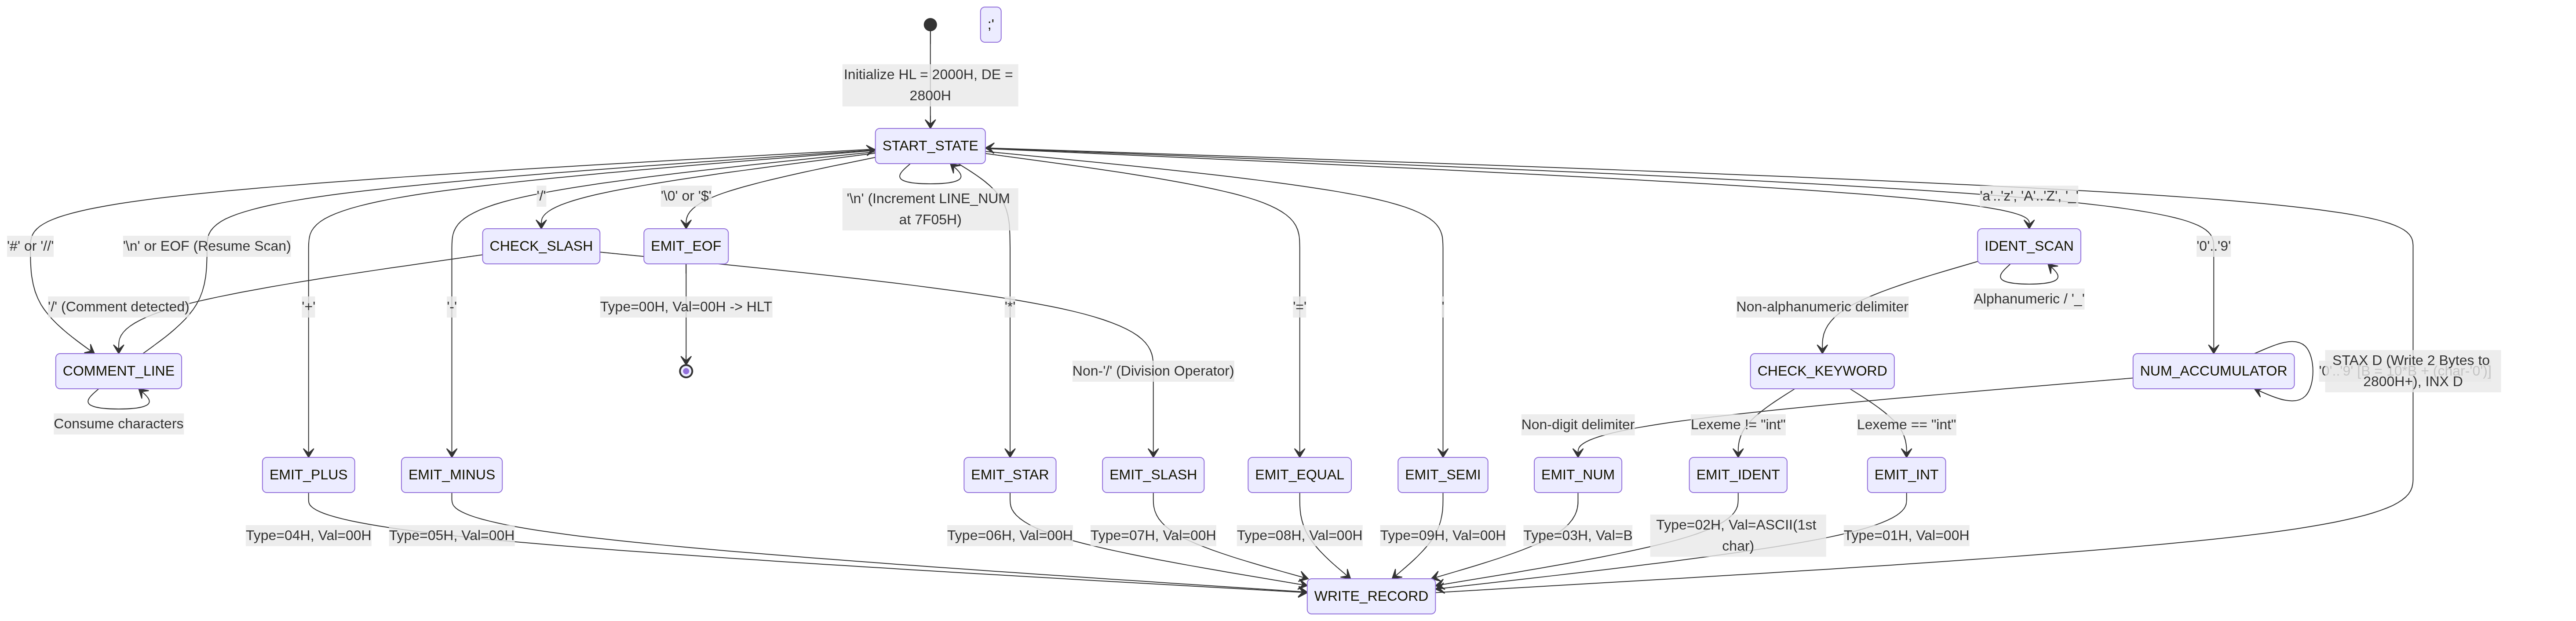
\includegraphics[width=0.92\textwidth,keepaspectratio]{mer1.png}}
    \caption{NFA State Transition Diagram for MiniC Token Recognition}
    \label{fig:nfa}
\end{figure}

\begin{table}[H]
\centering
\small
\caption{NFA State Transitions and Token Actions}
\label{tab:nfa_matrix}
\begin{tabularx}{\textwidth}{|l|l|X|l|}
\hline
\rowcolor[gray]{0.92}
\textbf{Current State} & \textbf{Input Character} & \textbf{Engine Action} & \textbf{Next State / Token} \\
\hline
\texttt{S0 (Start)} & Space, Tab, CR & Advance read pointer (\texttt{INX H}) & \texttt{S0} (Skip) \\
\hline
\texttt{S0 (Start)} & \texttt{\textbackslash n} (Newline) & Increment line counter at \texttt{7F05H} & \texttt{S0} \\
\hline
\texttt{S0 (Start)} & \texttt{\#} or \texttt{//} & Discard characters until newline & \texttt{S\_COM} $\rightarrow$ \texttt{S0} \\
\hline
\texttt{S0 (Start)} & \texttt{'0'} \dots \texttt{'9'} & $B = \text{char} - \texttt{'0'}$ & \texttt{S\_NUM} \\
\hline
\texttt{S0 (Start)} & \texttt{a-z, A-Z, \_} & Buffer character in \texttt{CUR\_NAME} & \texttt{S\_ID} \\
\hline
\texttt{S0 (Start)} & \texttt{+, -, *, /, =, ;} & Set token type, set value byte to \texttt{00H} & \texttt{EMIT\_OP} \\
\hline
\texttt{S0 (Start)} & \texttt{\textbackslash 0} or \texttt{\$} & Set type \texttt{00H}, value \texttt{00H}, halt & \texttt{EMIT\_EOF} \\
\hline
\texttt{S\_NUM} & \texttt{'0'} \dots \texttt{'9'} & $B = (B \times 10) + (\text{char} - \texttt{'0'})$ & \texttt{S\_NUM} \\
\hline
\texttt{S\_NUM} & Non-digit delimiter & Emit $\langle\texttt{03H}, B\rangle$, step back pointer & \texttt{Accept (TOK\_NUM)} \\
\hline
\texttt{S\_ID} & Alphanumeric / \texttt{\_} & Append character to \texttt{CUR\_NAME} & \texttt{S\_ID} \\
\hline
\texttt{S\_ID} & Non-alphanumeric & Check \texttt{"int"}: emit \texttt{TOK\_INT} or \texttt{TOK\_IDENT} & \texttt{Accept} \\
\hline
\end{tabularx}
\end{table}

% ------------------------------------------------------------------------------
% 6. INTEL 8085 IMPLEMENTATION
% ------------------------------------------------------------------------------
\section{Intel 8085 Assembly Implementation}

\subsection*{Memory Map}
\begin{table}[H]
\centering
\small
\caption{Intel 8085 Memory Layout Map}
\label{tab:memory}
\begin{tabularx}{\textwidth}{|c|c|l|X|}
\hline
\rowcolor[gray]{0.92}
\textbf{Address Range} & \textbf{Size} & \textbf{Region Name} & \textbf{Description / Purpose} \\
\hline
\texttt{2000H -- 27FFH} & 2 KB & \textbf{Source Buffer}  & Input MiniC ASCII text (null-terminated). \\
\hline
\texttt{2800H -- 2FFFH} & 2 KB & \textbf{Token Stream}   & Output sequential array of 2-byte token records. \\
\hline
\texttt{4000H -- 43FFH} & 1 KB & \textbf{Lexer Program}  & Machine code binary (Execution starts at \texttt{4000H}). \\
\hline
\texttt{7F00H -- 7F10H} & 17 B & \textbf{State Variables}& Internal pointers, counters, and temporary buffers. \\
\hline
\texttt{FFFFH (down)}  & --   & \textbf{Call Stack}     & Descending stack initialized with \texttt{LXI SP, 0FFFFH}. \\
\hline
\end{tabularx}
\end{table}

\begin{figure}[H]
    \centering
    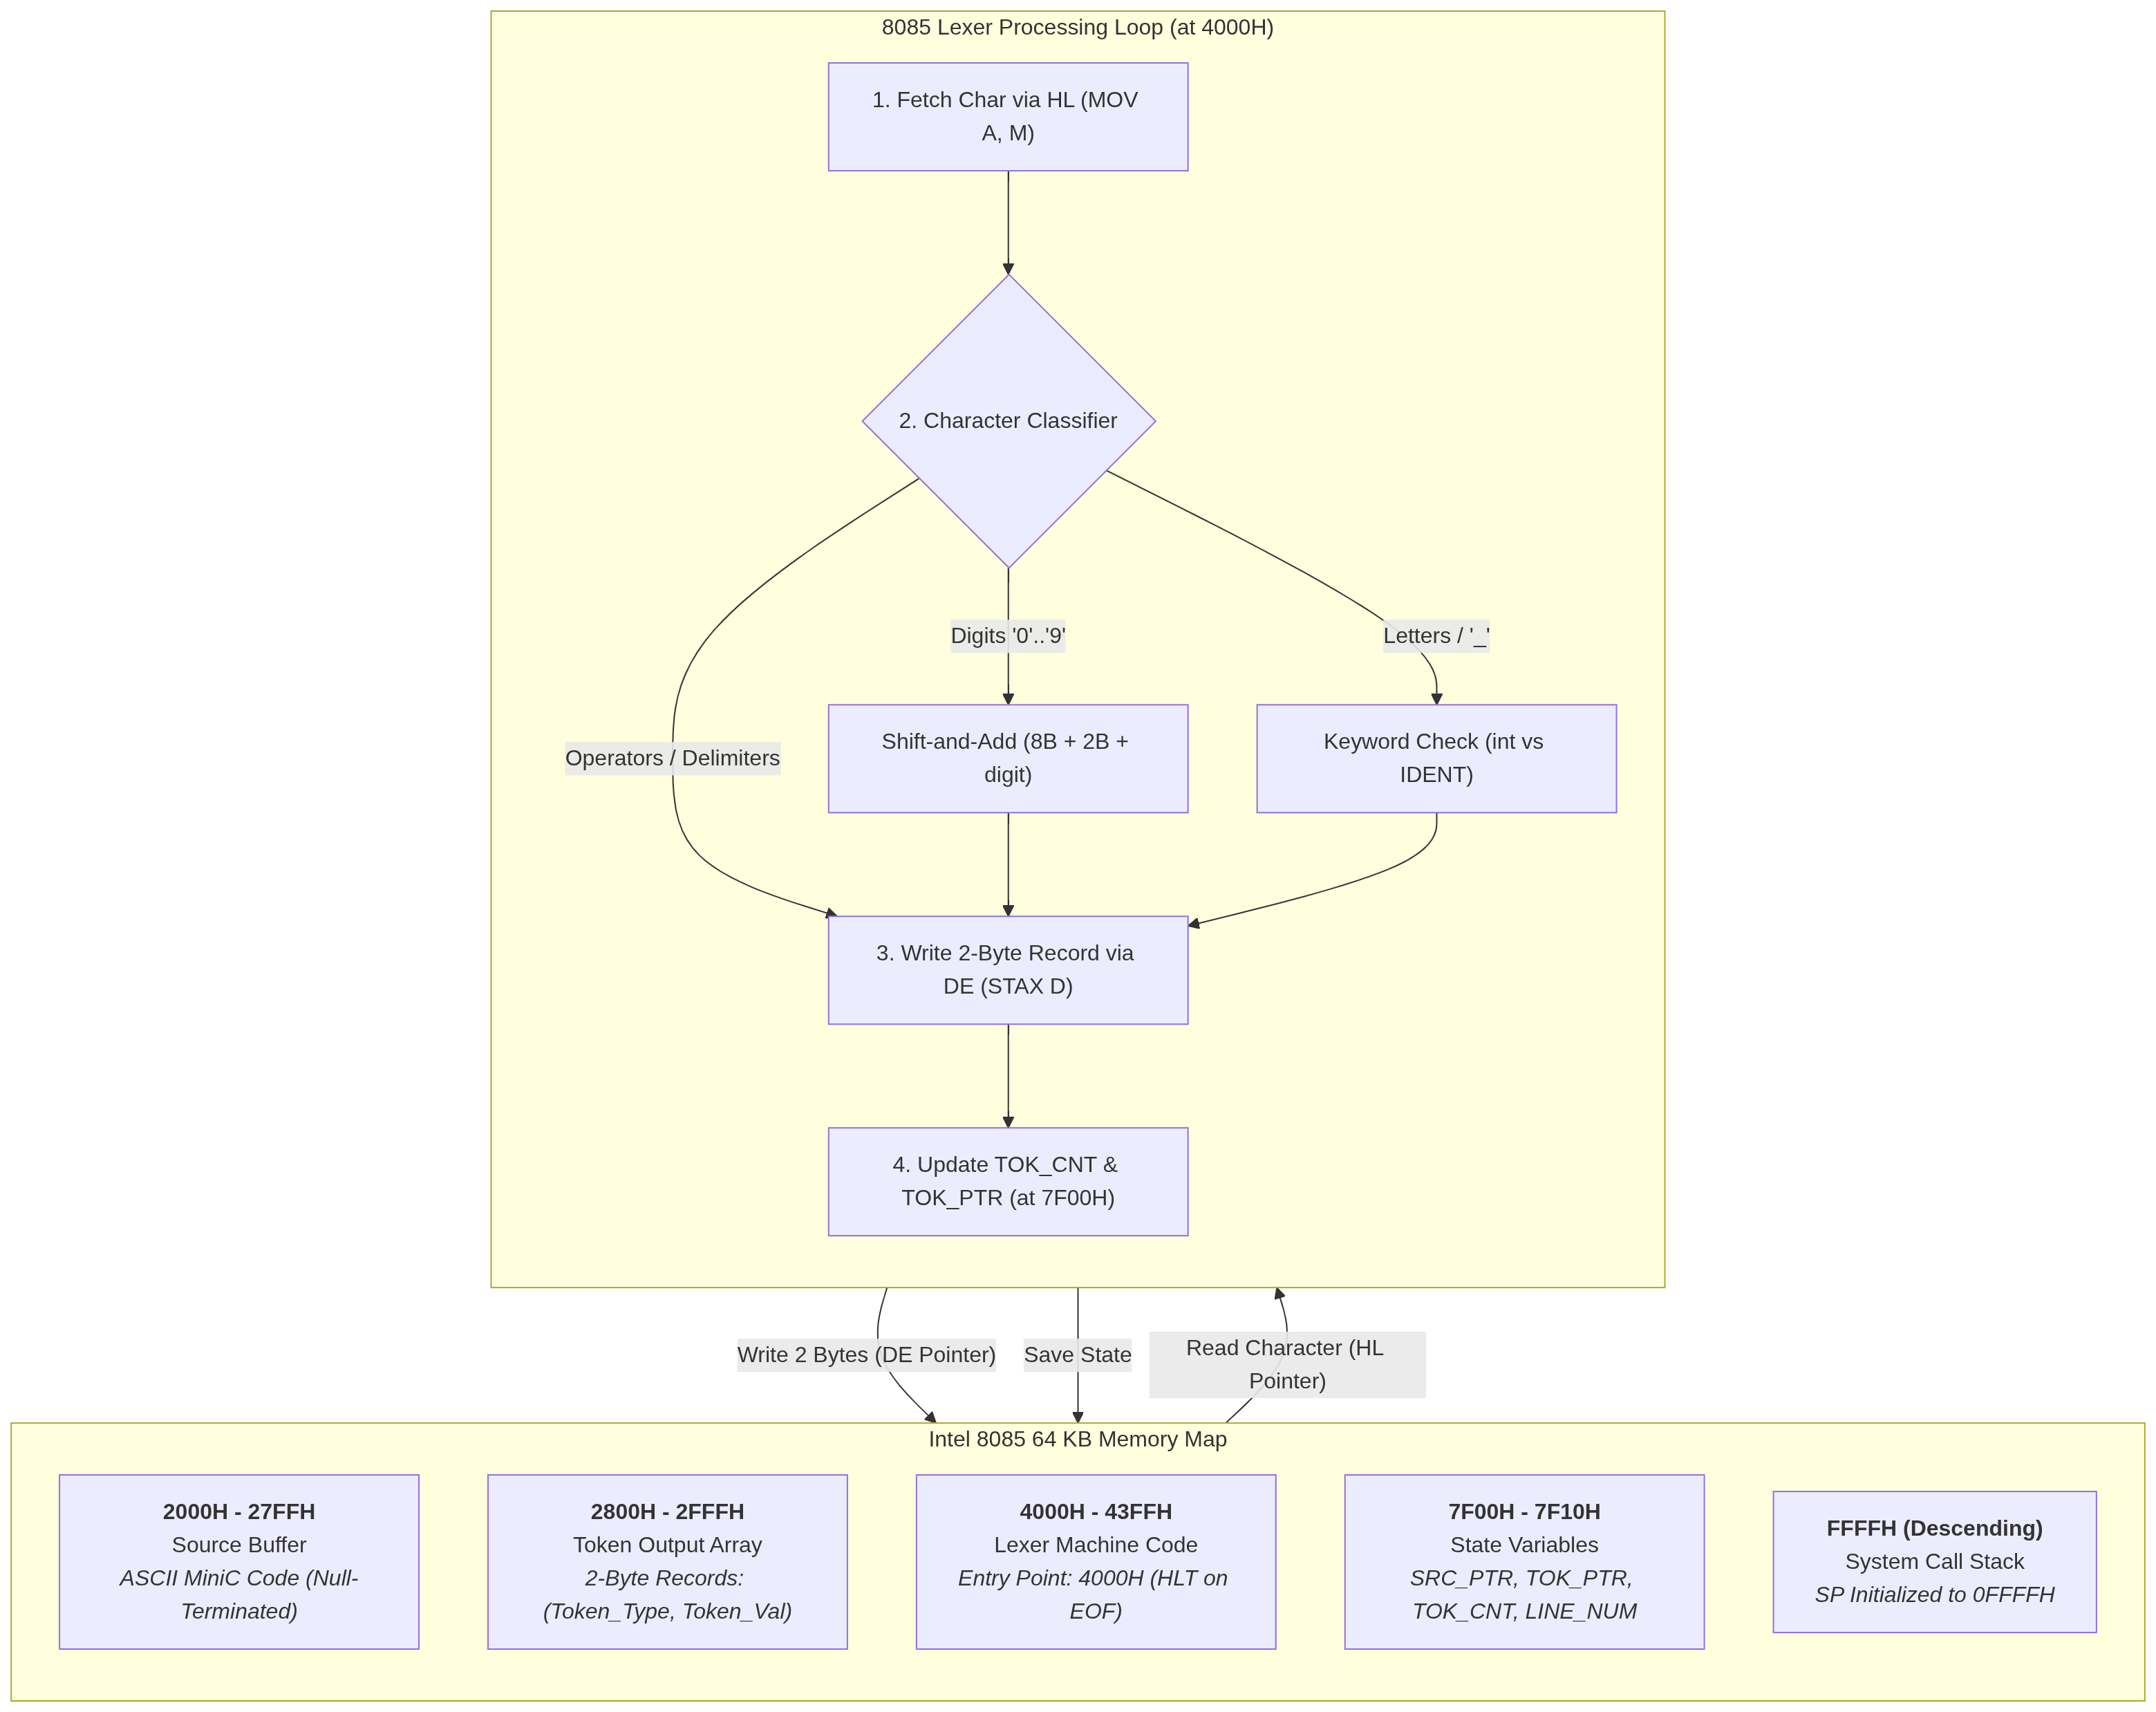
\includegraphics[width=0.78\textwidth,keepaspectratio]{mer2.png}
    \caption{Intel 8085 Lexer Processing Flow and Memory Map}
    \label{fig:memory_flow}
\end{figure}

\subsection*{Register Allocation}
\begin{table}[H]
\centering
\small
\caption{8085 Register Allocation Scheme}
\label{tab:registers}
\begin{tabularx}{\textwidth}{|c|l|X|}
\hline
\rowcolor[gray]{0.92}
\textbf{Register / Pair} & \textbf{Assigned Role} & \textbf{Functional Purpose} \\
\hline
\textbf{\texttt{HL} Pair} & Source Read Pointer (\texttt{SRC\_PTR}) & Points to current input character at \texttt{2000H+}. \\
\hline
\textbf{\texttt{DE} Pair} & Token Write Pointer (\texttt{TOK\_PTR}) & Points to current output record at \texttt{2800H+}. \\
\hline
\textbf{\texttt{B} Register} & Numeric Accumulator & Holds intermediate base-10 value during decimal conversion. \\
\hline
\textbf{\texttt{C} Register} & Scratch / Arithmetic Temp & Temporary register during shift-and-add multiplication. \\
\hline
\textbf{\texttt{A} (Accumulator)} & ALU / Comparators & Character comparisons (\texttt{CPI}), arithmetic, and flags. \\
\hline
\textbf{Flags (\texttt{CY}, \texttt{Z})} & Classifier Status & Outputs from character and keyword checking routines. \\
\hline
\end{tabularx}
\end{table}

\subsection*{Core Subroutines}
\begin{itemize}[itemsep=2pt, topsep=2pt]
    \item \textbf{Shift-and-Add Multiplication (\texttt{MULT10}):} Since the 8085 has no \texttt{MUL} instruction, multi-digit accumulation uses $10 \times B = (8 \times B) + (2 \times B) = (B \ll 3) + (B \ll 1)$.
    \item \textbf{Character Classifiers (\texttt{IS\_LET}, \texttt{IS\_DIG}):} Uses \texttt{CPI} and the Carry flag to classify digits and identifier characters.
    \item \textbf{Keyword Check (\texttt{CK\_INT}):} Checks if the buffered string is \texttt{"int"}. Emits \texttt{TOK\_INT} (\texttt{01H}) if matched, else \texttt{TOK\_IDENT} (\texttt{02H}).
    \item \textbf{State Variables at \texttt{7F00H}:} Tracks \texttt{SRC\_PTR} (\texttt{7F00H}), \texttt{TOK\_PTR} (\texttt{7F02H}), \texttt{TOK\_CNT} (\texttt{7F04H}), \texttt{LINE\_NUM} (\texttt{7F05H}), and \texttt{CUR\_NAME} (\texttt{7F08H}).
\end{itemize}

% ------------------------------------------------------------------------------
% 7. FLEX IMPLEMENTATION
% ------------------------------------------------------------------------------
\section{Flex Implementation}
The Flex scanner (\texttt{lexer.l}) matches tokens declaratively and writes identical 2-byte token entries into simulated 8085 memory:

\begin{lstlisting}[language=C]
"int"           { record_token(TOK_INT,   "TOK_INT",   yytext, 0x00); return TOK_INT; }
"+"             { record_token(TOK_PLUS,  "TOK_PLUS",  yytext, 0x00); return TOK_PLUS; }
"-"             { record_token(TOK_MINUS, "TOK_MINUS", yytext, 0x00); return TOK_MINUS; }
"*"             { record_token(TOK_STAR,  "TOK_STAR",  yytext, 0x00); return TOK_STAR; }
"/"             { record_token(TOK_SLASH, "TOK_SLASH", yytext, 0x00); return TOK_SLASH; }
"="             { record_token(TOK_EQUAL, "TOK_EQUAL", yytext, 0x00); return TOK_EQUAL; }
";"             { record_token(TOK_SEMI,  "TOK_SEMI",  yytext, 0x00); return TOK_SEMI; }
[0-9]+          { record_token(TOK_NUM,   "TOK_NUM",   yytext, (unsigned char)atoi(yytext)); return TOK_NUM; }
[a-zA-Z_][a-zA-Z0-9_]* { record_token(TOK_IDENT, "TOK_IDENT", yytext, (unsigned char)yytext[0]); return TOK_IDENT; }
\end{lstlisting}

% ------------------------------------------------------------------------------
% 8. WORKED EXAMPLE & VERIFICATION TRACE
% ------------------------------------------------------------------------------
\section{Worked Example and Verification Trace}

\subsection*{Sample Program}
The reference MiniC program loaded at address \texttt{2000H}:
\begin{lstlisting}
int a;
int b = 5;
int c = a * b + 3;
int d;
d = c - b * 2;
\end{lstlisting}

\subsection*{Extracted Token Stream at Address \texttt{2800H}}
Table~\ref{tab:trace} shows all 28 tokens extracted and the exact 2-byte memory output generated at address \texttt{2800H}:

\begin{table}[H]
\centering
\small
\caption{Token Output Stream and 8085 Memory Map}
\label{tab:trace}
\begin{tabularx}{\textwidth}{|c|c|l|c|c|X|}
\hline
\rowcolor[gray]{0.92}
\textbf{Token \#} & \textbf{Address} & \textbf{Token Name} & \textbf{Type Byte} & \textbf{Value Byte} & \textbf{Lexeme / Description} \\
\hline
\#0  & \texttt{2800H} & \texttt{TOK\_INT}   & \texttt{01H} & \texttt{00H} & Keyword \texttt{int} \\
\hline
\#1  & \texttt{2802H} & \texttt{TOK\_IDENT} & \texttt{02H} & \texttt{61H} & Identifier \texttt{a} (ASCII \texttt{61H}) \\
\hline
\#2  & \texttt{2804H} & \texttt{TOK\_SEMI}  & \texttt{09H} & \texttt{00H} & Semicolon \texttt{;} \\
\hline
\#3  & \texttt{2806H} & \texttt{TOK\_INT}   & \texttt{01H} & \texttt{00H} & Keyword \texttt{int} \\
\hline
\#4  & \texttt{2808H} & \texttt{TOK\_IDENT} & \texttt{02H} & \texttt{62H} & Identifier \texttt{b} (ASCII \texttt{62H}) \\
\hline
\#5  & \texttt{280AH} & \texttt{TOK\_EQUAL} & \texttt{08H} & \texttt{00H} & Assignment \texttt{=} \\
\hline
\#6  & \texttt{280CH} & \texttt{TOK\_NUM}   & \texttt{03H} & \texttt{05H} & Number \texttt{5} (Value \texttt{05H}) \\
\hline
\#7  & \texttt{280EH} & \texttt{TOK\_SEMI}  & \texttt{09H} & \texttt{00H} & Semicolon \texttt{;} \\
\hline
\#8  & \texttt{2810H} & \texttt{TOK\_INT}   & \texttt{01H} & \texttt{00H} & Keyword \texttt{int} \\
\hline
\#9  & \texttt{2812H} & \texttt{TOK\_IDENT} & \texttt{02H} & \texttt{63H} & Identifier \texttt{c} (ASCII \texttt{63H}) \\
\hline
\#10 & \texttt{2814H} & \texttt{TOK\_EQUAL} & \texttt{08H} & \texttt{00H} & Assignment \texttt{=} \\
\hline
\#11 & \texttt{2816H} & \texttt{TOK\_IDENT} & \texttt{02H} & \texttt{61H} & Identifier \texttt{a} \\
\hline
\#12 & \texttt{2818H} & \texttt{TOK\_STAR}  & \texttt{06H} & \texttt{00H} & Multiplication \texttt{*} \\
\hline
\#13 & \texttt{281AH} & \texttt{TOK\_IDENT} & \texttt{02H} & \texttt{62H} & Identifier \texttt{b} \\
\hline
\#14 & \texttt{281CH} & \texttt{TOK\_PLUS}  & \texttt{04H} & \texttt{00H} & Addition \texttt{+} \\
\hline
\#15 & \texttt{281EH} & \texttt{TOK\_NUM}   & \texttt{03H} & \texttt{03H} & Number \texttt{3} (Value \texttt{03H}) \\
\hline
\#16 & \texttt{2820H} & \texttt{TOK\_SEMI}  & \texttt{09H} & \texttt{00H} & Semicolon \texttt{;} \\
\hline
\#17 & \texttt{2822H} & \texttt{TOK\_INT}   & \texttt{01H} & \texttt{00H} & Keyword \texttt{int} \\
\hline
\#18 & \texttt{2824H} & \texttt{TOK\_IDENT} & \texttt{02H} & \texttt{64H} & Identifier \texttt{d} (ASCII \texttt{64H}) \\
\hline
\#19 & \texttt{2826H} & \texttt{TOK\_SEMI}  & \texttt{09H} & \texttt{00H} & Semicolon \texttt{;} \\
\hline
\#20 & \texttt{2828H} & \texttt{TOK\_IDENT} & \texttt{02H} & \texttt{64H} & Identifier \texttt{d} \\
\hline
\#21 & \texttt{282AH} & \texttt{TOK\_EQUAL} & \texttt{08H} & \texttt{00H} & Assignment \texttt{=} \\
\hline
\#22 & \texttt{282CH} & \texttt{TOK\_IDENT} & \texttt{02H} & \texttt{63H} & Identifier \texttt{c} \\
\hline
\#23 & \texttt{282EH} & \texttt{TOK\_MINUS} & \texttt{05H} & \texttt{00H} & Subtraction \texttt{-} \\
\hline
\#24 & \texttt{2830H} & \texttt{TOK\_IDENT} & \texttt{02H} & \texttt{62H} & Identifier \texttt{b} \\
\hline
\#25 & \texttt{2832H} & \texttt{TOK\_STAR}  & \texttt{06H} & \texttt{00H} & Multiplication \texttt{*} \\
\hline
\#26 & \texttt{2834H} & \texttt{TOK\_NUM}   & \texttt{03H} & \texttt{02H} & Number \texttt{2} (Value \texttt{02H}) \\
\hline
\#27 & \texttt{2836H} & \texttt{TOK\_SEMI}  & \texttt{09H} & \texttt{00H} & Semicolon \texttt{;} \\
\hline
\#28 & \texttt{2838H} & \texttt{TOK\_EOF}   & \texttt{00H} & \texttt{00H} & End of Stream (\texttt{\textbackslash 0}) \\
\hline
\end{tabularx}
\end{table}

\subsection*{Final State at Address \texttt{7F00H}}
Upon program halt (\texttt{HLT}):
\begin{itemize}[itemsep=2pt, topsep=2pt]
    \item \texttt{7F00H - 7F01H} (\texttt{SRC\_PTR}): \texttt{203CH} (Points past null terminator).
    \item \texttt{7F02H - 7F03H} (\texttt{TOK\_PTR}): \texttt{283AH} (Points after \texttt{TOK\_EOF}).
    \item \texttt{7F04H} (\texttt{TOK\_CNT}): \texttt{1CH} (28 decimal tokens).
    \item \texttt{7F05H} (\texttt{LINE\_NUM}): \texttt{07H} (Line 7 reached).
\end{itemize}

% ------------------------------------------------------------------------------
% 9. CONCLUSION
% ------------------------------------------------------------------------------
\section{Conclusion}
The MiniC Lexical Analyzer was implemented in both Intel 8085 Assembly and Flex. The assembly version runs directly on bare-metal 8085 hardware within $\sim 280$ bytes of memory, while the Flex version provides rapid declarative verification. Both versions were verified to produce identical 2-byte token streams and memory dumps starting at address \texttt{2800H}.

\end{document}
